
\chapter{Simulaciones}
\label{cap:simulaciones}

A lo largo de este capítulo veremos con detalle las simulaciones que se han realizado del modelo visto en \ref{sub:modelo}. Reproduciremos el comportamiento individual de cada célula y veremos, una vez completada la simulación, el efecto global de estas decisiones individuales.

El código propuesto se ha realizado en Matlab y puede verse en ... anexo? 


\section{Modelo simplificado}

Para las simulaciones hemos optado por un sistema simplificado al propuesto en \ref{sub:modelo}, de tal manera que el número de parámetros sea suficiente para no perder la esencia del modelo pero no muy elevado para no distraer al lector con notación engorrosa. Siguiendo con la notación de \ref{sub:modelo}, asumiremos $k=2$. Es decir, hay dos tipos de receptores: \textit{p} (de proliferación) y \textit{d} (de muerte) que controlan
la evolución de los inhibidores de ciclo y apóptosis.

De esta manera y asumiendo que los receptores de proliferación de las células T efectoras se expresan siguiendo las señales TCR, que autorregulan su expresión y que inducen la producción de receptores tipo \textit{d}, tenemos que las ecuaciones \ref{sist_inhib} y \ref{sist_recep} pueden escribirse como:

\begin{equation}
	\label{sist9_simplif}
	\left\{ \begin{array}{l}
	\dot{c}(t) = -\mu_{pc}p(t) \\
	\dot{a}(t) = -\mu_{da}d(t)  \\
	\dot{p}(t) = \lambda_{Tp}r_{T}(t) - \lambda_{pp}p(t) \\
	\dot{d}(t) = \lambda_{pd}p(t) \\
	\\
	c(0)=c_0 \\
	a(0)=a_0 \\
	p(0)=p_0 \\
	d(0)=d_0 
	\end{array}
	\right.
\end{equation}

Así mismo, hemos simulado de manera conjunta este Sistema \ref{sist9_simplif}, la Ecuación \ref{sist_pat_T} y la dinámica de las células T de memoria. Esta última viene dada por el mismo Sistema \ref{sist9_simplif}, en el que se ha tenido en cuenta que $d=0$, puesto que nos centramos solamente en el inhibidor del ciclo celular (recordemos que las células T de memoria no mueren durante la \textit{contracción clonal}). Así las cosas, las ecuacines que rigen el algoritmo de decisión para células T de memoria viene dado por: 

\begin{equation}
	\label{sist15_simplif}
	\left\{ \begin{array}{l}
	\dot{c}(t) = -\mu_{pc}p(t) \\
	\dot{p}(t) = \lambda_{Tp}r_{T}(t) - \lambda_{pp}p(t) \\
	\\
	c(0)=c_0 \\
	p(0)=p_0 \\
	\end{array}
	\right.
\end{equation}


A la hora de realizar la simulación de este modelo hay que tener especial cuidado con la elección de los parámetros y tener en cuenta que muchos de ellos son específicos para un patógeno concreto, lo que hace que obtengamos un resultado u otro dependiendo de estos. A continuación se muestra la Tabla \ref{tabla:param} con los parámetros elegidos para nuestra simulación:
HAY QUE ACTULIZAR LOS PARÁMETROS DE ESTA TABLA, NO SON LOS FINALES

\begin{table}[h]
	\begin{center}
	\begin{tabular}{|l|l|l|}
		\hline 
		\multirow{9}{*}{}  &  $t_{cycle} = 0.15$ & Duración de la fase de ciclo.\\ \cline{2-3} 
		& $t_{apo} = 0,2$  & Duración de la fase de apóptosis.  \\ \cline{2-3} 
		& $t_{next} = 0,3$  & Duración del paso en la simulación. \\ \cline{2-3} 
		& $a_0 = 0,3$ & Cantidad inicial de Bcl-2 para células T efectoras. \\ \cline{2-3} 
		Variables & $c_0 = 0,08$  & Cantidad inicial de Rb para células T efectoras. \\ \cline{2-3} 
		& $c_0^{mem} = 0,04$  & Cantidad inicial de Rb para células T de memoria. \\ \cline{2-3} 
		& $N_{ini} = 25$ & Número inicial de células T naïve.  \\ \cline{2-3} 
		& $Y_{ini} = 5$  & Número inicial de moléculas del patógeno. \\ \cline{2-3} 
		& $r_p, r_d = 0$ & Número inicial de receptores de membrana $p$ y $d$. \\ \hline
		\multirow{2}{*}{}  & $\alpha = 10$ & Tasa de proliferación. \\ \cline{2-3} 
		Patógeno & $\beta = 0,1$ & Tasa de muerte por linfocito. \\ \hline
		\multirow{5}{*}{}  & $\lambda_{pd} = 0,04$  & Tasa de cambio del receptor $R_d$ por cada señal $R_p$. \\ \cline{2-3} 
		 & $\lambda_{Tp} = 6*10^{-5}$ & Tasa de cambio del receptor $R_p$ por cada señal del TCR.  \\ \cline{2-3} 
		Células T & $\lambda_{pp} = 0,5*10^{-5}$ & Tasa de cambio del receptor $R_p$ por cada señal $R_p$. \\ \cline{2-3} 
		efectoras& $\mu_{pc} = 0,4$ & Tasa de cambio de Rb por cada señal del TCR.  \\ \cline{2-3} 
		& $\mu_{da} = 3,5$ & Tasa de cambio de Bcl-2 por cada señal del TCR. \\ \hline
		\multirow{4}{*}{}  & $\lambda_{Tp}^{mem} = 10^{-6}$ & Igual que $\lambda_{Tp}$, para células T de memoria. \\ \cline{2-3} 
		Células T & $\lambda_{pp}^{mem} = 2*10^{-2}$ & Igual que $\lambda_{pp}$, para células T de memoria.  \\ \cline{2-3} 
		de memoria & $\mu_{pc}^{mem} = 0,3$ & Igual que $\mu_{pc}$, para células T de memoria. \\ \cline{2-3} 
		\hline
	\end{tabular}
\caption{Tabla de variables y parámetros.}
\label{tabla:param}
\end{center}
\end{table}


\section{Pseudocódigo}

Con ánimo de aclarar los aspectos más básicos de la implementación, se presenta un pseudocódigo (ver Algoritmo \ref{algo:pseudocodigo}) de la misma. El código completo puede verse en PONER ANEXO O DONDE VAYA.


\begin{algorithm}
	\caption{Algoritmo de la decisión. Células T.}
	\label{algo:pseudocodigo}
	\begin{algorithmic}[1]
		
		% ENTRADA / SALIDA
		
		\State Inicialización de parámetros según \ref{tabla:param}
		\State $t = 0;$ \Comment{t será el tiempo por el que vamos simulando}
		
		\While{ $t\ < \ T_{final}$}
		  
		\State $Y = Y_{init}*e^{t*(\alpha - N*\beta)};$ \Comment{Calculamos Y con la solución explícita de \ref{sist_pat_T}}
		
		\For{$nCell; nCell++; N$} \Comment{Para cada célula T de la población}
			\State $ r_{T}=\rho*Y;$ \Comment{Ecuación \ref{ec:rhotau}}
			\If{$efectora(nCell)$} \Comment{Si es una célula T efectora}
				\State Se resuelve \ref{sist9_simplif}
				\If{$a \leq 0 $}
					\State La célula $nCell$ se elimina de la población
				\ElsIf{$c \leq 0$}
					\State La célula $nCell$ se divide
					\State Las condiciones iniciales de las células hijas vienen determinadas por $a_0, c_0$ y \ref{sist:div_sim}
				\EndIf
			
			\ElsIf{$memoria(nCell)$} \Comment{Si es una célula T de memoria}
				\State Se resuelve \ref{sist15_simplif}
				\If{$c \leq 0$}
					\State La célula $nCell$ se divide siguiendo el mismo procedimiento que la división de una célula T efectora. 
				\EndIf
			\EndIf
		\EndFor
		
		\State Se actualiza el número de células de la población.
		\State $t = t + t_{next};$
		
		\EndWhile
		
	\end{algorithmic}
\end{algorithm}

En este pseudocódigo hemos omitido que cuando las condiciones son $a > 0$ y $c > 0$, en el caso de las células T efectoras y $c > 0$, en el caso de las células T de memoria, la célula permanece en la fase de decisión pero actualiza sus condiciones para la siguiente iteración según los resultados que ha obtenido en la iteración actual. También hay que tener en cuenta que la división celular y el proceso de apóptosis no se llevan a cabo de manera inmediata, tienen un tiempo $t_{cycle}$ y $t_{apo}$, respectivamente, por lo que el número total de células en la población debe actualizarse cuando toque y no antes de que ninguna de estas dos fases haya finalizado. Otro aspecto que hemos supuesto es que el parámetro $\gamma$ que aparecía en la Ecuación \ref{ec:rhotau} es $\gamma = 1$. Es decir, suponemos que todo encuentro del TCR de la célula T con el antígeno va a desencadenar una activación. El parámetro $\rho$ debe ser calculado de tal manera que todas las células T tengan las mismas posibilidades a la hora de ``obtener su parte de patógeno'', en la implementación real se usó un vector de números aleatorios entre 0 y 1 normalizado por el número de células T.

Buena parte de la notación usada en el Algoritmo \ref{algo:pseudocodigo} ya ha sido introducida a lo largo de este trabajo, pero volvemos a insistir en que $Y$ representa el número de moléculas del patógeno, mientras que $N$ la cantidad total de células T, incluyendo las efectoras y las de memoria. Sin embargo, en la implementación real, en la línea 4 del pseudocódigo, el $N$ utilizado es solamente el número total de células T efectoras, sin contar las de memoria \footnote{Esto se ha hecho así porque el proceso que siguen las célualas T de memoria es más complejo que lo que se recoge en el modelo. Estas células al cabo de un tiempo se desactivan y para que tengan un efecto sobre el patógeno deben volver a activarse. Para intentar hacer el modelo lo más sencillo posible se ha optado por hacer que las únicas células que combaten al patógeno sean las T efectoras}.

\section{Resultados y análisis}

En esta sección  veremos los resultados de algunas simulaciones. La primera de ellas, Figura \ref{fig:intolerance}, muestra la simulación correspondiente a la elección de parámetros que se recoge en la Tabla \ref{tabla:param}. Estamos ante un caso de intolerancia al patógeno, puesto que las células T son capaces de eliminarlo por completo. 
Veámoslo con más detalle: el patógeno, representado con un línea roja, crece rápidamente, debido a la elección de una tasa de crecimiento, $\alpha$, elevada. Una vez que las células T son conscientes de la rápida proliferación de un agente no deseado, su número comienza a crecer. Sin embargo, como ya habíamos comentado anteriormente, esto se produce con cierto retraso tras la aparición del patógeno. Lo que estamos describiendo es la conocida \textit{expansión clonal}. Este crecimiento de células T provoca que el término que acompaña a $\beta$ en la Ecuación \ref{sist_pat_T} comience a ser más grande que el acompañado por $\alpha$ en esta misma ecuación, provocando así que la derivada de $y$ se haga negativa y, por tanto, el número de moléculas del patógeno comience a decrecer. Debemos mencionar que el número de células T necesarias para eliminar el patógeno viene regulado por el parámetro $\beta$, si este fuera más grande, es decir, las células T fueran más dañinas con el patógeno, veríamos una curva azul con un máximo mas pequeño que el de la Figura \ref{fig:intolerance}. (EN REALIDAD EN ESTA FIGURA LA GRÁFICA ESTÁ NORMALIZADA, SERÍA MEJOR PONER LA OTRA SIN NORMALIZAR?)Pero ¿qué pasaría si la fuerza de estas células T no fuera suficiente? El patógeno crecería de manera exponencial, a mucha más velocidad que las células T, de forma que estas no podrían llegar a acabar con él. 

Prestemos atención ahora al comportamiento de las células T de memoria. Por la sección anterior, ya sabíamos que las células T efectoras y las de memoria iban a constituir poblaciones distintas, puesto que las ecuaciones que rigen sus dinámicas son distintas. La principal diferencia es que las células T de memoria no se suicidan una vez el patógeno ha desaparecido, sabemos que permanecen con la información necesaria para atacar al patógeno más rápidamente en caso de reaparición. Vemos cómo estas células de memoria aumentan su población tras la aparición del patógeno, no vemos un crecimiento tan grande. Su población queda reducida a un $5-10\%$ de la población de células T.


\begin{figure}[t]
	\centering
	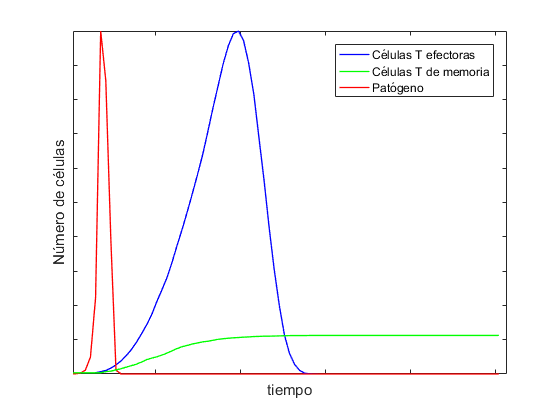
\includegraphics[width=0.7\textwidth]{Imagenes/Simulaciones/intolerance}
	\caption{Simulación: caso de intolerancia al patógeno.}
	\label{fig:intolerance}
\end{figure}
